\subsubsection{Renderer}
\label{sec:renderer}
\hspace{\parindent} The renderer uses \hyperref[context]{\ref*{context} Context} that provides global properties of this renderer.\\
Despite the \hyperref[sec:headset]{\ref*{sec:headset} Headset} is not responsible for the \hyperref[sec:rendering_process]{\ref*{sec:rendering_process} Rendering Process}, that class has a big influence on the renderer, as our engine is designed for virtual reality purposes, we decided that headset's swapchain has a priority over window's swapchain due to that rendering depends on the image created by the headset (for an instance from the user experience it can be noticed by not having anything displayed on the window if a headset stays in standby mode). Therefore, \texttt{Headset} is explained here instead of having separated dedicated section.\\ Graphical presentation of the relations in the renderer portrays \hyperref[fig:renderer]{the followed image}.\\
The same applies \texttt{MirroView} class that is used as an intermediate layer of abstraction between \hyperref[window]{\ref*{window} \texttt{Window} class}, and the renderer.
\label{fig:renderer}
\begin{figure}[H]
  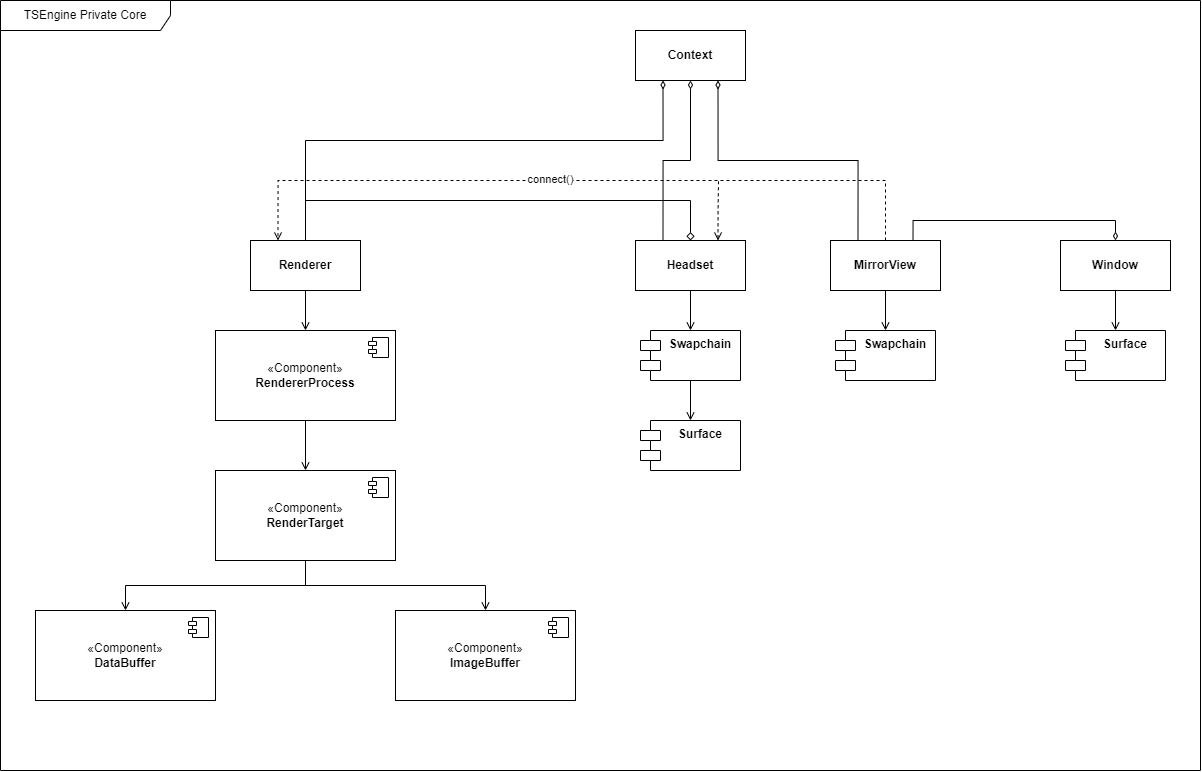
\includegraphics[width=\linewidth]{renderer.png}
  \caption{Renderer}
\end{figure}
We can distinguish the front-end of the renderer being the part of ECS - \hyperref[sec:renderer_system]{\ref*{sec:renderer_system}. ECS Renderer System}, but also back-end in classes:
\begin{itemize}
    \item \texttt{Renderer}\\
    Comprehensive component of the engine core that manages various aspects of the rendering pipeline in a Vulkan environment that plays a role of back-end of the renderer. It orchestrates render processes, manages Vulkan resources like command pools and descriptor pools, and handles different pipelines for rendering. The class's structure emphasizes controlled resource management, synchronization, and the ability to handle multiple frames in flight, which are key elements in high-performance graphics applications.
    \item Renderer components:
    \begin{itemize}
    \item \texttt{DataBuffer}\\
    It encapsulates Vulkan buffer handling, abstracting details such as buffer creation, memory management, and data transfer.
    \item \texttt{ImageBuffer}\\
    It is designed for encapsulation of the creation and management of Vulkan images, device memory allocations, and image views,
    \item \texttt{Pipeline}\\
    This class encompass the complexity of Vulkan many different stages and settings, from shader stages to fixed-function state like blending, depth testing, providing a more streamlined interface for setting up and using these pipelines in rendering operations. 
    \item \texttt{RenderTarget}
    It is designed to encapsulate the concept of a render target in Vulkan. It manages the creation and lifecycle of a framebuffer and associated image views, which are fundamental to rendering operations. The framebuffer combines color and depth/stencil attachments, which are used during a render pass. 
    \item \texttt{RendererProcess}
    It manages uniform data for objects and lights, handles synchronization primitives, and maintains various Vulkan objects essential for rendering operations.
    \end{itemize}
    \item Renderer-related:
    \begin{itemize}
        \item \texttt{Headset}\\
        \label{sec:headset}
        \item \texttt{MirrorView}\\
        Despite being strongly linked with OpenXR \texttt{MirrorView} is the part of the renderer. 
    \end{itemize}
\end{itemize}